%15 min preso!
\documentclass[xcolor=table,aspectratio=169]{beamer}
\usepackage{beamerthemesplit}
\usepackage{wrapfig}
\usetheme{SPbGU}
\usepackage{pdfpages}
\usepackage{amsmath}
\usepackage{cmap}
\usepackage[T2A]{fontenc}
\usepackage[utf8]{inputenc}
\usepackage[english]{babel}
\usepackage{indentfirst}
\usepackage{amsmath}
\usepackage{tikz}
\usepackage{multirow}
\usepackage[noend]{algpseudocode}
\usepackage{algorithm}
\usepackage{algorithmicx}
\usepackage{fancyvrb}
\usepackage{hyperref} 
\usetikzlibrary{calc}
\usetikzlibrary{shapes}
\usetikzlibrary{arrows,automata}
\usetikzlibrary{positioning}
\usetikzlibrary{fit}
\usetikzlibrary{shapes.callouts}
\usetikzlibrary{shapes.misc}
\usepackage{xparse}

\usepackage{etoolbox,refcount}
\usepackage{multicol}

\usepackage{fontawesome5}
\usepackage{fontawesome}

\usepackage{tabularx}
\newcolumntype{Y}{>{\raggedleft\arraybackslash}X}

\renewcommand{\thealgorithm}{}

\newtheorem{mytheorem}{Theorem}
\renewcommand{\thealgorithm}{}

\newcommand{\tikzmark}[1]{\tikz[overlay,remember picture] \node (#1) {};}
\def\Put(#1,#2)#3{\leavevmode\makebox(0,0){\put(#1,#2){#3}}}

\newcommand{\ltz}{$< 1$}

\tikzset{
    state/.style={
           rectangle,
           rounded corners,
           draw=black, very thick,
           minimum height=2em,
           inner sep=2pt,
           text centered,
           },
}

\tikzset{
    invisible/.style={opacity=0,text opacity=0},
    visible on/.style={alt=#1{}{invisible}},
    alt/.code args={<#1>#2#3}{%
      \alt<#1>{\pgfkeysalso{#2}}{\pgfkeysalso{#3}} % \pgfkeysalso doesn't change the path
    },
}

\tikzset{cross/.style={cross out, draw=black, minimum size=2*(#1-\pgflinewidth), inner sep=0pt, outer sep=0pt, ultra thick},
%default radius will be 1pt. 
cross/.default={1pt}}

\NewDocumentCommand{\mycallout}{r<> O{opacity=0.8,text opacity=1} m m m}{%
\tikz[remember picture, overlay]\node[align=center, fill=cyan!20, text width=#5cm,
#2,visible on=<#1>, rounded corners,
draw,rectangle callout,anchor=pointer,callout relative pointer={(290:0.5cm)}]
at (#3) {#4};
}

\NewDocumentCommand{\mycalloutR}{r<> O{opacity=0.8,text opacity=1} m m m}{%
\tikz[remember picture, overlay]\node[align=center, fill=cyan!20, text width=#5cm,
#2,visible on=<#1>, rounded corners,
draw,rectangle callout,anchor=pointer,callout relative pointer={(30:0.8cm)}]
at (#3) {#4};
}


%callout relative pointer={(230:0.5cm)}]

\newcounter{countitems}
\newcounter{nextitemizecount}
\newcommand{\setupcountitems}{%
  \stepcounter{nextitemizecount}%
  \setcounter{countitems}{0}%
  \preto\item{\stepcounter{countitems}}%
}
\makeatletter
\newcommand{\computecountitems}{%
  \edef\@currentlabel{\number\c@countitems}%
  \label{countitems@\number\numexpr\value{nextitemizecount}-1\relax}%
}
\newcommand{\nextitemizecount}{%
  \getrefnumber{countitems@\number\c@nextitemizecount}%
}
\newcommand{\previtemizecount}{%
  \getrefnumber{countitems@\number\numexpr\value{nextitemizecount}-1\relax}%
}
\makeatother    
\newenvironment{AutoMultiColItemize}{%
\ifnumcomp{\nextitemizecount}{>}{3}{\begin{multicols}{2}}{}%
\setupcountitems\begin{itemize}}%
{\end{itemize}%
\unskip\computecountitems\ifnumcomp{\previtemizecount}{>}{3}{\end{multicols}}{}}


\beamertemplatenavigationsymbolsempty

\title[GraphBLAS \& Graph databases]{Graph Analysis Team Introduction}
\subtitle{Experience in GraphBLAS and Graph Databases}
\institute[PL\&T@SPbSU]{
Saint Petersburg State University
}

% То, что в квадратных скобках, отображается в левом нижнем углу.
\author[Semyon Grigorev]{Semyon Grigorev}

\date{April 30, 2022}

\begin{document}
{
\begin{frame}[fragile]
  \begin{table}
  \centering
  
\includegraphics[height=1.5cm]{pictures/SPbGU_Logo.png}  
  \end{table}
  \titlepage
\end{frame}
}

\begin{frame}[fragile]
  \frametitle{Group Info}  
  \begin{itemize}
      \item Established in 2012
      \item Lead: Semyon Grigorev
      \begin{itemize}
        \item PhD (2016), Associate professor (2016, SPbSU)
        \item dblp: \href{https://dblp.org/pid/181/9903.html}{https://dblp.org/pid/181/9903.html}
        \item h-index (scopus): 5
        \item \href{s.v.grigoriev@spbu.ru}{s.v.grigoriev@spbu.ru}
      \end{itemize}
      \item PhD students: 2
      \item Master students: 5
      \item Bachelor students: 6
      \item Publications
      \begin{itemize}
        \item Total: > 30
        \item Scopus: 25 
      \end{itemize}
    \end{itemize}
\end{frame}

\begin{frame}[fragile]
  \frametitle{Research Area}
  \begin{itemize}
    \item High-performance graph analysis
    \begin{itemize}
      \item GraphBLAS-based algorithms design, implementation and evaluation
      \item Portable multi-GPGPU implementation of GraphBALS-like API
      \item GraphBLAS API analysis
    \end{itemize} 
    \pause
    \item Formal Language Constrained Path Querying (FLPQ)
    \begin{itemize}
      \item New algorithms development
      \item Complexity analysis
      \item New classes of languages investigation
      \item High performance algorithms implementation and evaluation 
    \end{itemize}    
  \end{itemize}
\end{frame}

\begin{frame}[fragile]
  \frametitle{GraphBLAS API}
  \begin{columns}[t]
    \begin{column}{0.45\textwidth}
  \begin{itemize}
    \item Graph-matrix duality
    \item Operations over matrices and vectors
    \begin{itemize}
      \item Parametrized by semiring-like structures
      \item Based on sparse data structures
      \item Highly parallel
    \end{itemize}    
  \end{itemize}
\end{column}
\pause
\begin{column}{0.55\textwidth}
  \begin{itemize}
  \item High-performance implementations
    \begin{itemize}
      \item SuiteSparse:GraphBLAS\footnotemark[1]: pure C
      \item GraphBLAST\footnotemark[2]: GPGPU, Cuda C
      \item Huawei's GraphBLAS\footnotemark[3]: C++
      \item \ldots
    \end{itemize}
  \end{itemize}
\end{column}
\end{columns}
\pause
\begin{itemize}
  \item More information on GraphBLAS
  \begin{itemize}
    \item Home page: \url{https://graphblas.org/}
    \item GraphBLAS-related resources: \url{https://graphblas.org/GraphBLAS-Pointers/}
    \item Introduction to GraphBLAS: \url{http://mit.bme.hu/~szarnyas/grb/graphblas-introduction.pdf}     
  \end{itemize}    
\end{itemize}
\footnotetext[1]{\url{https://github.com/DrTimothyAldenDavis/GraphBLAS}}
\footnotetext[2]{\url{https://github.com/gunrock/graphblast}}
\footnotetext[3]{\url{https://gitee.com/CSL-ALP/graphblas}}
\end{frame}


\begin{frame}[fragile]
  \frametitle{GraphBLAS Applications}  
  \begin{columns}[t]
    \begin{column}{0.5\textwidth}
  \begin{itemize}
    \item BFS-like algorithms
    \begin{itemize}
      \item BFS: levels, parents, multiple sources
      \item SSSP
      \item \ldots
    \end{itemize}
    \item Graph clustering
  \end{itemize}
 \end{column}
\begin{column}{0.5\textwidth}
  \begin{itemize}
    \item Transitive closure based algorithms
    \begin{itemize}
      \item APSP      
      \item \ldots
    \end{itemize}
    \item Triangle counting    
    \item \ldots
  \end{itemize}
\end{column}
\end{columns}
\pause
\vspace{0.5cm}
\begin{itemize}
    \item LAGraph: collection of GraphBLAS-based algorithms  
  \begin{itemize}
    \item GitHub: \url{https://github.com/GraphBLAS/LAGraph}
    \item Latest report: \url{https://arxiv.org/pdf/2104.01661.pdf}
  \end{itemize}
\end{itemize}
\end{frame}

\begin{frame}[fragile]
  \frametitle{Formal Language Constrained Path Querying (FLPQ)}
    \begin{itemize}
      \item A way to use formal languages to specify constraints on paths            
      \begin {itemize}
        \item Regular path querying (RPQ): regular expressions as constraints
        \item Context-free path querying (CFPQ): context-free grammars as constraints
      \end{itemize}
    \pause    
    \item Applications 
    \begin{itemize}
      \item Graph analysis
      \item Interprocedural static code analysis
      \item Graph database querying
    \end{itemize}
  \end{itemize}
\end{frame}

\begin{frame}[fragile]
  \frametitle{Our Results: GraphBLAS Implementation}
    \begin{itemize}
      \item Tools
      \begin{itemize}
        \item \href{https://github.com/JetBrains-Research/spbla}{SPbLA: library of GPGPU-powered sparse boolean linear algebra operations}            
        \item \href{https://github.com/JetBrains-Research/spla}{Spla: sparse linear algebra framework for multi-GPU computations based on OpenCL}        
      \end{itemize}
      \pause
      \item Papers
      \begin{itemize}
        \item SPbLA: The Library of GPGPU-Powered Sparse Boolean Linear Algebra Operations (GrAPL@IPDPS)
      \end{itemize} 
    \end{itemize}
\end{frame}

\begin{frame}[fragile]
  \frametitle{GraphBLAS Implementation Evaluation: SPbLA\footnote{More details: \url{https://github.com/JetBrains-Research/spbla\#performance}}}
  \vspace{-0.8cm}
  \tikzmark{xxx}{}  
    \begin{center}      
        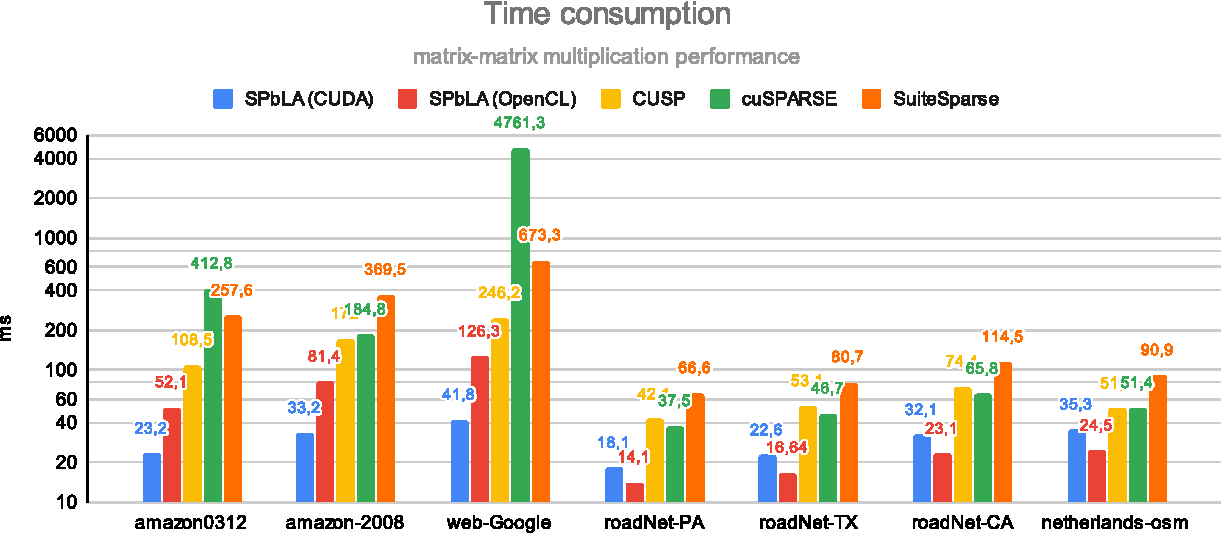
\includegraphics[width = \textwidth]{pictures/mxm-perf-time-crop.pdf}
    \end{center}    
    \pause
  \onslide<2>{\tikz[overlay,remember picture]{
    \draw[draw=red,thick,double,fill opacity=0.2] ($ (xxx) + (2.6,-1.2)$) rectangle ($ (xxx) + (7.3,-1.65)$);
    \draw[draw=red,thick,double,fill opacity=0.2] ($ (xxx) + (1.6,-4.8)$) rectangle ($ (xxx) + (2.4,-6.5)$);
    \draw[draw=red,thick,double,fill opacity=0.2] ($ (xxx) + (3.5,-4.5)$) rectangle ($ (xxx) + (4.3,-6.5)$);
    \draw[draw=red,thick,double,fill opacity=0.2] ($ (xxx) + (5.4,-4.2)$) rectangle ($ (xxx) + (6.3,-6.5)$);
    \draw[draw=red,thick,double,fill opacity=0.2] ($ (xxx) + (7.4,-5.3)$) rectangle ($ (xxx) + (8.2,-6.5)$);
    \draw[draw=red,thick,double,fill opacity=0.2] ($ (xxx) + (9.3,-5.3)$) rectangle ($ (xxx) + (10.1,-6.5)$);
    \draw[draw=red,thick,double,fill opacity=0.2] ($ (xxx) + (11.2,-5.1)$) rectangle ($ (xxx) + (12.0,-6.5)$);
    \draw[draw=red,thick,double,fill opacity=0.2] ($ (xxx) + (13.15,-5.1)$) rectangle ($ (xxx) + (13.95,-6.5)$);
    }}  
\end{frame}

\begin{frame}[fragile]
  \frametitle{GraphBLAS Implementation Evaluation: Spla}
  \tikzmark{zzz}{}
  \begin{table}[tbp]
    \caption{Triangles counting algorithms evaluation results. Time in milliseconds (lower is better).} 
    \begin{center}
        \begin{tabular}{|l|r|r|r|r|r|r|r|}
        \hline
        \multicolumn{3}{|c|}{Dataset} & \multicolumn{3}{c|}{Nvidia} & \multicolumn{2}{c|}{Intel} \\
        %\cline{2-6}
        \hline
         Name & \#V & \#E & GR & GB & SP & SS & SP \\
        \hline
        \hline        
        \rowcolor{black!10} coAuthorsCiteseer & 227.3K &   1.6M &   2.1 &    2.0 &    9.5 &    17.5 &    64.9 \\
        \rowcolor{black!2 } coPapersDBLP      & 540.4K &  30.4M &   5.7 &   94.4 &  201.9 &   543.1 &  1537.8 \\
        \rowcolor{black!10} roadNet-CA        &   1.9M &   5.5M &  34.3 &    5.8 &   16.1 &    47.1 &   357.6 \\
        \rowcolor{black!2 } com-Orkut         &     3M &   234M & 218.1 & 1583.8 & 2407.4 & 23731.4 & 15049.5 \\
        \rowcolor{black!10} cit-Patents       &   3.7M &  16.5M &  49.7 &   52.9 &   90.6 &   698.3 &   684.1 \\
        \rowcolor{black!2 } soc-LiveJournal   &   4.8M &  68.9M &  69.1 &  449.6 &  673.9 &  4002.6 &  3823.9 \\
        \hline
        \hline
        \multicolumn{6}{l}{Tools: Gunrock (GR), GraphBLAST (GB), SuiteSparse (SS), Spla (SP)} \\
        \end{tabular}
        \label{results}
    \end{center}
    \end{table}
    \pause
  \onslide<2>{\tikz[overlay,remember picture]{\draw[draw=red,thick,double,fill opacity=0.2] ($ (zzz) + (7.6,-2.2)$) rectangle ($ (zzz) + (11.9,-5.7)$);}}
  \onslide<3>{\tikz[overlay,remember picture]{\draw[draw=red,thick,double,fill opacity=0.2] ($ (zzz) + (6.3,-3.7)$) rectangle ($ (zzz) + (11.9,-4.2)$);
                                              \draw[draw=red,thick,double,fill opacity=0.2] ($ (zzz) + (6.3,-4.7)$) rectangle ($ (zzz) + (11.9,-5.2)$);}}
  \onslide<4>{\tikz[overlay,remember picture]{\draw[draw=red,thick,double,fill opacity=0.2] ($ (zzz) + (11.8,-4.2)$) rectangle ($ (zzz) + (15.2,-5.7)$);}}                                              
\end{frame}

\begin{frame}[fragile]
  \frametitle{Our Results: Graph Databases Extensions with CFPQ}
    \begin{itemize}
      \item Tools
      \begin{itemize}                
        \item \href{https://github.com/JetBrains-Research/GLL4Graph}{GLL4Graph: CFPQ for Neo4j}
        \item \href{https://github.com/YaccConstructor/RedisGraph}{CFPQ for RedisGraph}
      \end{itemize}
      \pause
      \item Papers
      \begin{itemize}                
        \item Multiple-Source Context-Free Path Querying in Terms of Linear Algebra (EDBT, Core A)
        \item Context-free path querying by matrix multiplication (GRADES-NDA@SIGMOD)
      \end{itemize} 
    \end{itemize}
\end{frame}

\begin{frame}[fragile]
  \frametitle{Graph Databases Extensions with CFPQ: Evaluation}

  \begin{center}      
    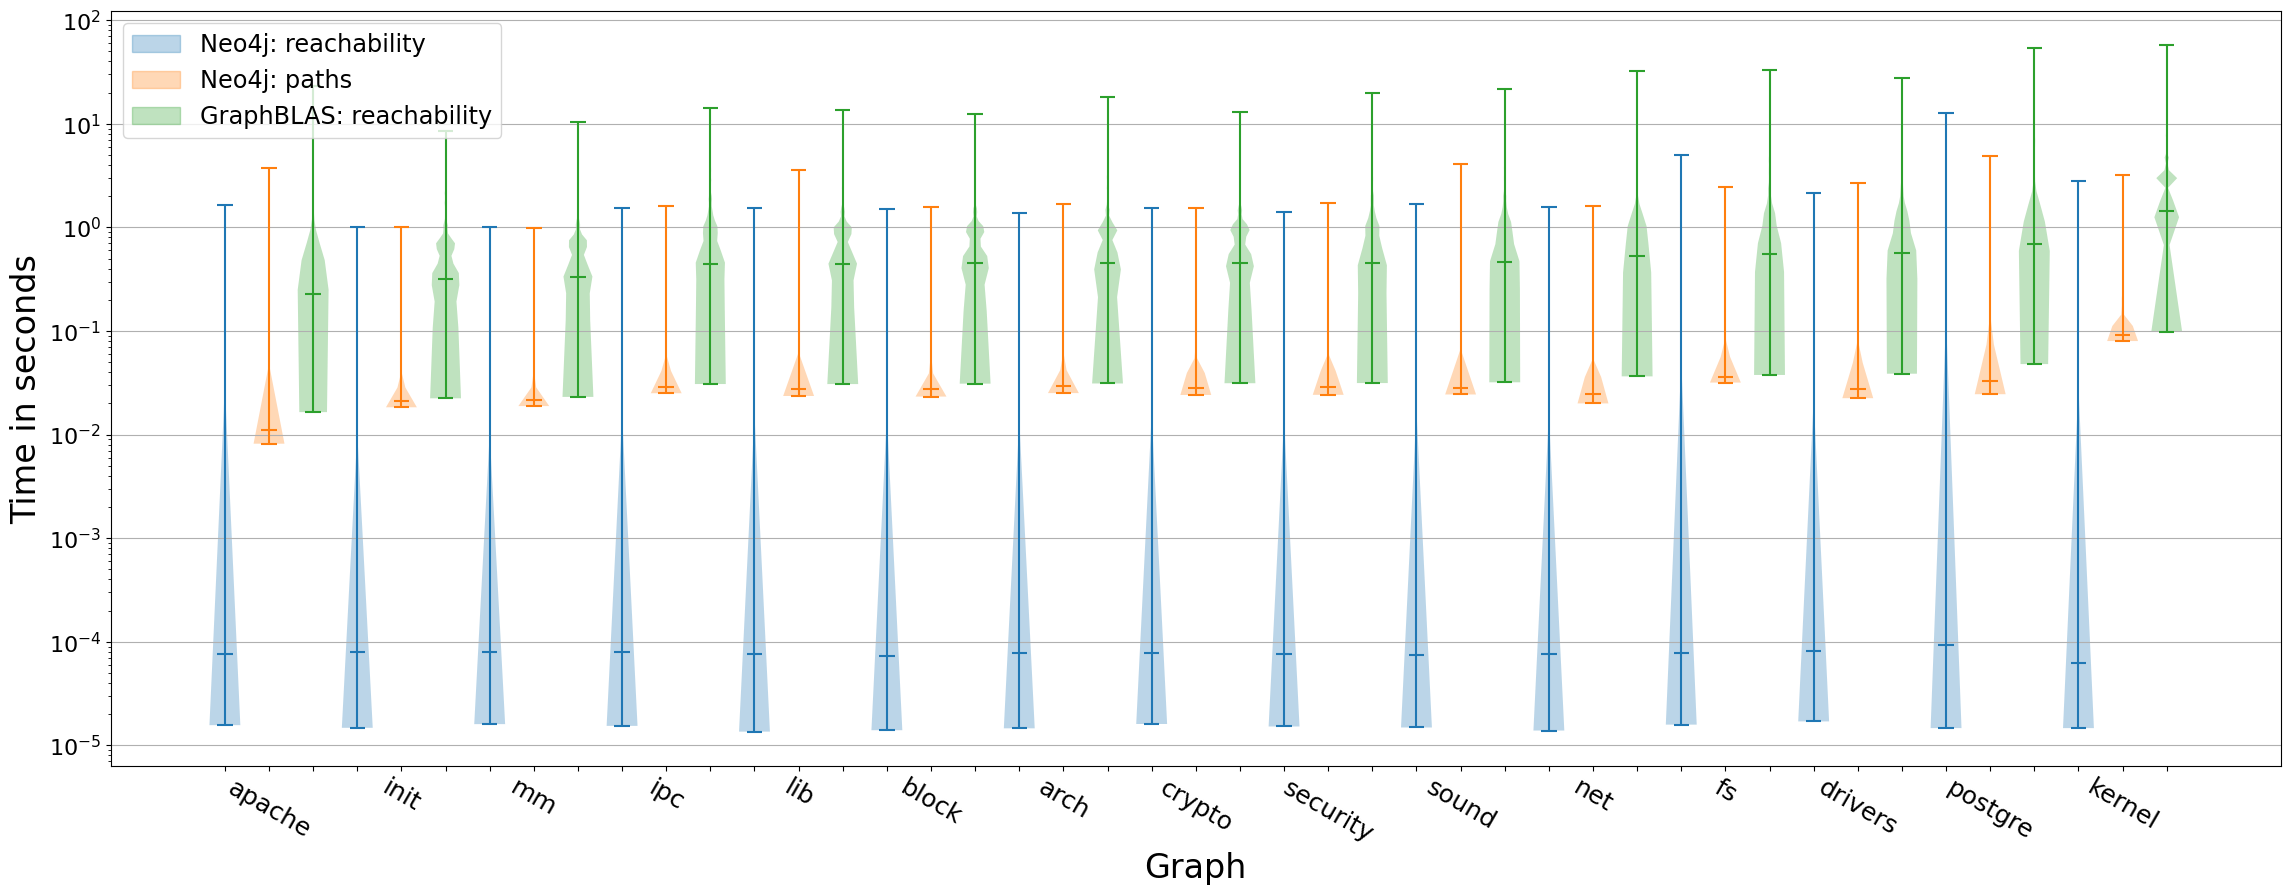
\includegraphics[width = \textwidth]{pictures/stat-m.png}
\end{center} 

    %{\tikz[overlay,remember picture]{\draw[draw=black,fill=white,fill opacity=1] (1.3,6.6) rectangle (3.9,6.35) node[align=left,pos=.5] {\tiny{Neo4j: reachability}};
    %                                 \draw[draw=black,fill=white,fill opacity=1] (1.3,6.35) rectangle (3.9,6.10) node[pos=.5] {\tiny{Neo4j: paths}};
    %                                 \draw[draw=black,fill=white,fill opacity=1] (1.3,6.10) rectangle (3.9,5.85) node[pos=.5] {\tiny{GraphBLAS: reachability}};
   % 
   % }}
\end{frame}

\begin{frame}[fragile]
  \frametitle{Our Results: FLPQ Algorithms Evaluation}
    \begin{itemize}
      \item Tools
      \begin{itemize}
        \item \href{https://github.com/JetBrains-Research/CFPQ_PyAlgo}{CFPQ\_PyAlgo: set of GraphBLAS-based FLPQ algorithms}
        \begin{itemize}  
          \item[\faCheck] GraphBLAS-based CFPQ algorithms
          \item[\faGears] GraphBLAS-based RPQ algorithms
          \item[\faGears] GraphBLAS-based MCFG-PQ algorithms
        \end{itemize} 
        \pause
        \item \href{https://github.com/JetBrains-Research/CFPQ_Data}{CFPQ\_Data: dataset for FLPQ algoriths evaluation}
        \begin{itemize}  
          \item[\faCheck] Graphs for CFPQ evaluation
          \item[\faGears] Graphs for RPQ evaluation
          \item[\faGears] Integration with LDBC Graphalytics
        \end{itemize} 
        \pause
        \item[\faGears] \href{https://github.com/JetBrains-Research/ldbc_graphalytics}{LDBC Graphalytics extension for evaluation of formal language constrained path querying}            
      \end{itemize}
      \pause
      \item Papers 
      \begin{itemize}        
        \item Evaluation of the context-free path querying algorithm based on matrix multiplication (GRADES-NDA@SIGMOD)
      \end{itemize} 
    \end{itemize}
\end{frame}


\end{document}
